\addsection{Pipeline samples} 
%
\noindent A good start for designing new pipelines
is to have a look at and take inspiration from the provided samples
available in ``data/pipes''. They describe how to use generic nodes
and show how to easily and quickly obtain multiple effects. This
section presents the samples.

\addsubsection{image-operators.gra}
%
\begin{figure}[htb]
  \centering 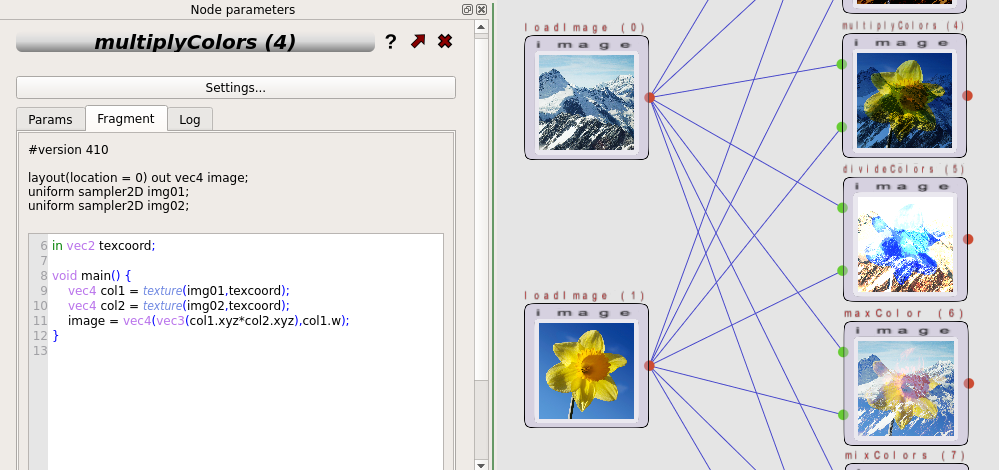
\includegraphics[width=\linewidth]{imgs/pipe-img-operators.png} 
  \caption{\label{fig:pipe-opp}The image operator pipeline example.}
\end{figure}
%
\noindent image-operators is the simplest pipeline and shows how to
combine two input images using simple image operators ($+,-,*,/,etc$).
Images are loaded with a ``loadImage'' node. All the combining
operations are done with some ``genericImage'' nodes
(Fig.~\ref{fig:pipe-opp}). In these nodes, the fragment shader is
executed independently on each image pixel. One can visualize the code
by double-clicking on a node and choosing the ``fragment'' tab in the
node interface. Of course, you can modify the settings and the code to
obtain your own desired effect. The only node containing a parameter
in these examples is the ``mixColors'' node that linearly interpolates
between 2 images based on a user-chosen value (in the ``Params'' tab
of the node interface).

\addsubsection{color-conversion.gra}
%
\begin{figure}[htb]
  \centering 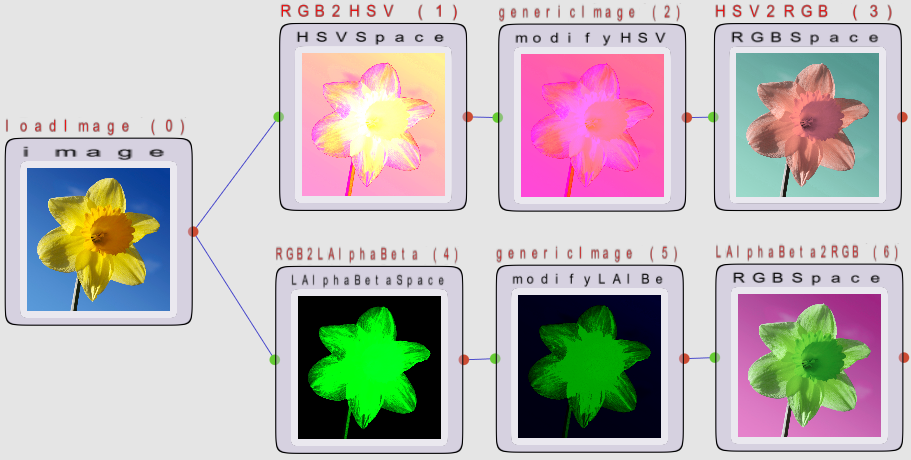
\includegraphics[width=\linewidth]{imgs/pipe-color-conv.png} 
  \caption{\label{fig:pipe-col-conv}The color conversion pipeline example.}
\end{figure}
%
\noindent This pipeline illustrates the use of color conversion nodes
to manipulate image colors (Fig.~\ref{fig:pipe-col-conv}). Except for the
loader, all nodes were created from the genericImage node. The top
row first convert an input RGB image into the HSV color space. A node
is then provided to control and manipulate HSV parameters (double
click on the ``modifyHSV'' node to try it via the interface). The last
node convert the HSV color back to the RGB color space, so that the
image can be displayed properly. The bottom row is similar, except
that colors are converted into the $L\alpha\beta$ color space.

\newpage
\addsubsection{image-filtering.gra}
%
\begin{figure}[b!]
  \centering 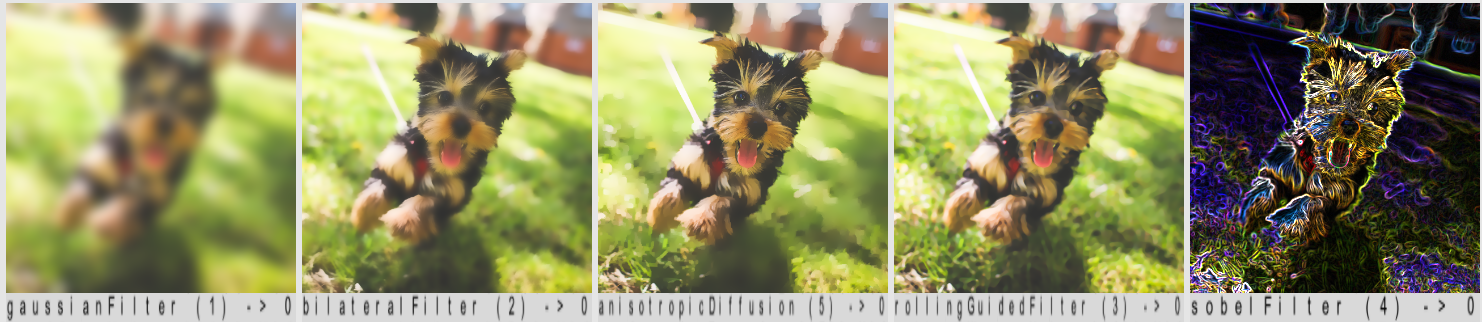
\includegraphics[width=\linewidth]{imgs/pipe-filter.png} 
  \caption{\label{fig:pipe-filter}Image filtering pipeline example.}
\end{figure}
%
\noindent This pipeline (Fig.~\ref{fig:pipe-filter}) illustrates the use of currently available
filtering nodes. The gaussian filter (left) was not implemented in a
generic node because it was optimized with a two-pass convolution kernel. The
bilateral filter (second) is based on a genericImage node. The
intensity and spatial sigma parameters can be controlled in the node
interface. The third example shows how a genericPingPong node was used
to obtain an anisotropic diffusion that iteratively diffuse colors
everywhere except on edges. The fourth example uses the same process
to obtain the rolling guided filter. The fifth example is based on a
genericImage node and detects edges using a Sobel filter.
\remark{Remark: citations for implemented papers are provided inside the node
  descriptions/helps.}

\addsubsection{curves-surfaces.gra}
\begin{figure}[htb]
  \centering 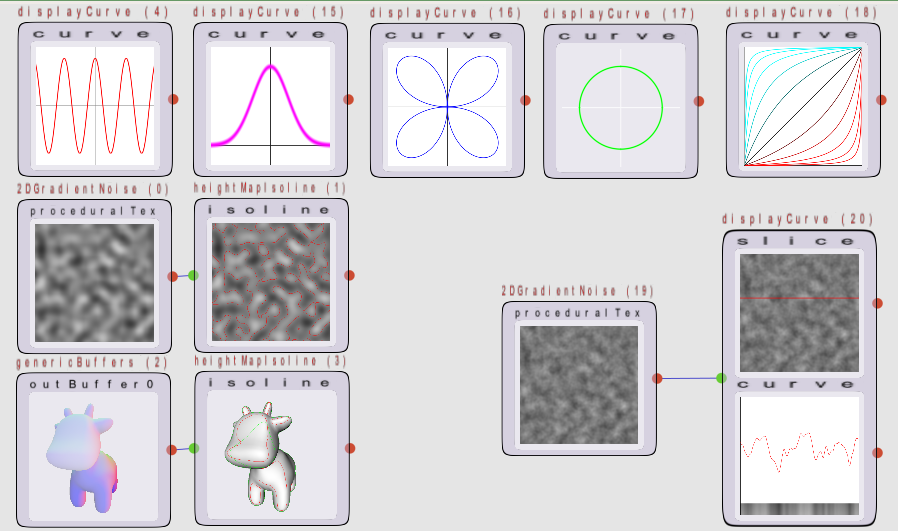
\includegraphics[width=\linewidth]{imgs/pipe-curves01.png} 
  \caption{\label{fig:pipe-curves}The curves examples.}
\end{figure}
%
\noindent This pipeline shows how to use nodes to visualize isolines,
curves and surfaces. The node ``displayCurve'' is based on a
genericImage node. It allows the user to easily modify a function
inside the GLSL code and visualize the resulting curve. The top row of
Fig.~\ref{fig:pipe-curves} shows some variations of this node, with
different functions, thicknesses and colors. To set your own curve,
open the ``fragment'' tab inside the node interface and modify the
equation inside the ``evalFunc'' function. Any parameter may be added
to the interface to control the curves in real-time, as shown in the
sine function node. \\ \\
%
In the bottom left of the figure, 2 examples of isoline visualization
are given. Again, this node is based on a genericImage node and might
be modified depending on user expectations. The first example shows
the isoline on a 2D noise texture. The isovalue can be controlled
inside the node interface. In the second example, the GLSL code was
slightly modified to simultaneously show 2 isoline curves, based on
2.5D information as input (surface slant in red and depth in Green).\\
\\
%
Finally, the bottom right example is a variation of the
``displayCurve'' node that was modified to display a slice of an input
image. This slice can be interactively changed in the viewer panel:
click on the slice and associated curve image and press ``space'' on
both of them. The two node outputs should thus appear in the viewer
panel. In this viewer, click on the slice image to select it and click
and drag vertically to control which slice to display in the curve
image.
%
\begin{figure}[htb]
  \centering 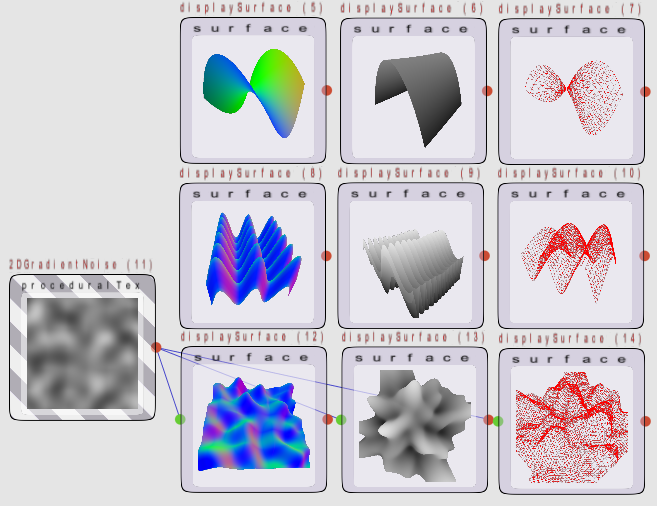
\includegraphics[width=\linewidth]{imgs/pipe-curves02.png} 
  \caption{\label{fig:pipe-surf}The surfaces examples.}
\end{figure}
% 
This pipeline also contain a set of nodes for visualizing surfaces, as
shown in Fig.~\ref{fig:pipe-surf}.  All these nodes are actually based
on variations of the ``displaySurface'' node, itself based on a
``genericGrid'' node. The user may modify the surface function by
editing the ``evalFunc'' function inside the vertex tab of the node
interface. From left to right, surfaces are visualized with their
normals (surface orientation), height and in wireframes. The top row
shows a quadratic function that can be manipulated with 2
parameters. The second row is a sinewave surface. The third one used a
heightfield as input to generate the 3D surface. The scale parameter
of the interface allows the height to be scaled manually. The camera
can be controlled in the viewer for each of this node.

\newpage
\addsubsection{flow-visualization.gra}
%
\begin{figure}[htb]
  \centering 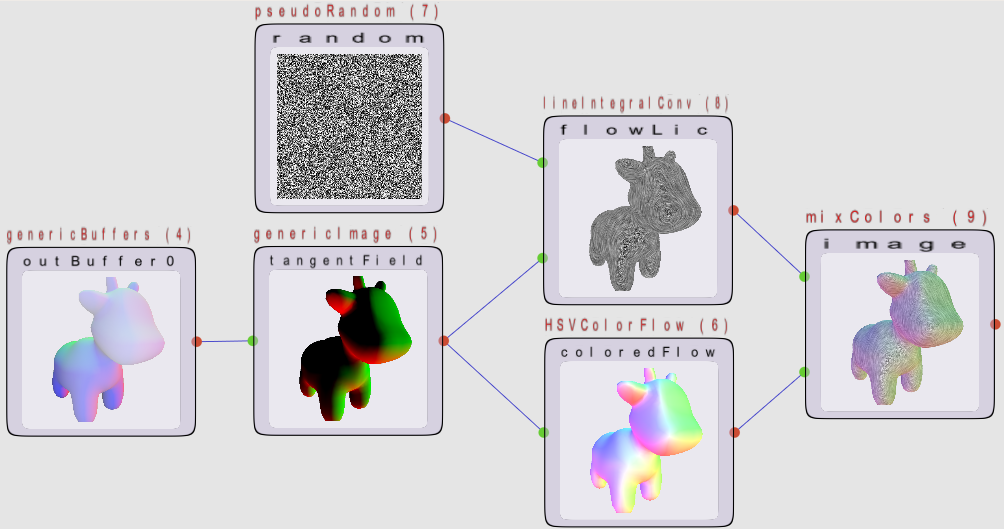
\includegraphics[width=\linewidth]{imgs/pipe-flows.png} 
  \caption{\label{fig:pipe-flow}Flow visualization pipeline example.}
\end{figure}
%
\noindent This pipeline (Fig~\ref{fig:pipe-flow}) illustrates the use of the
``lineIntegralConv'' and the ``HSVColorFlow'' nodes (based in generic
image nodes) to visualize a flow field. In this example, the flow is
obtained by computing the gradient flow of the surface. The line
integral convolution (LIC) blurs a texture (the noise in that case) in
the direction of the flow. This process is commonly used to visualize
flow field. The HSV color node has the same goal, but the input flow
direction is visualized with different hues and magnitude is related
to the color value. The last node on the right combines the flow to
obtain an original visualization.  The pipeline contains a second
example where an image is abstracted by applying a LIC, based on its
gradient flow.

\newpage
\addsubsection{laplacian-pyramid.gra}
\noindent The laplacian example (Fig.~\ref{fig:pipe-pyr}) shows how to use the
gaussian and laplacian pyramid nodes to decompose and modify the
frequency components of an image before rebuilding it. These pyramids
are all based on the ``genericPyramid'' node. In this example, small
scale details are enhanced before reconstructing the image. The last
node shows the resulting enhanced image by selecting the finest scale
of the pyramid (in a generic image node).

%
\begin{figure}[h!]
  \centering 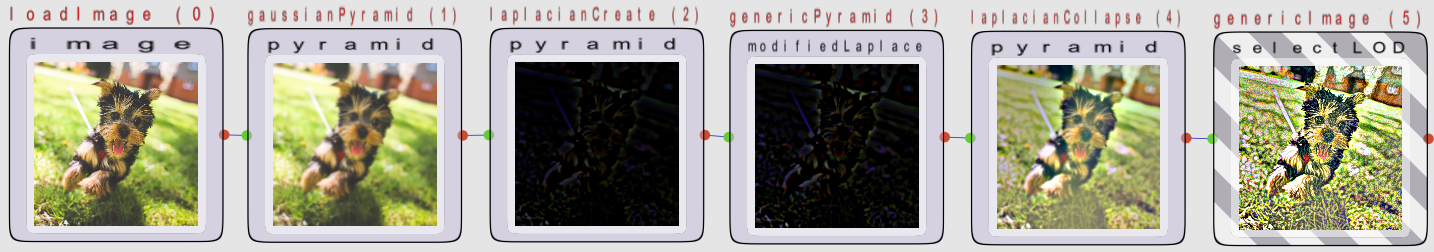
\includegraphics[width=\linewidth]{imgs/pipe-pyr.png} 
  \caption{\label{fig:pipe-pyr}Laplacian pyramid pipeline example.}
\end{figure}
%
\newpage

\addsubsection{global-values.gra}
%
\begin{figure}[htb]
  \centering 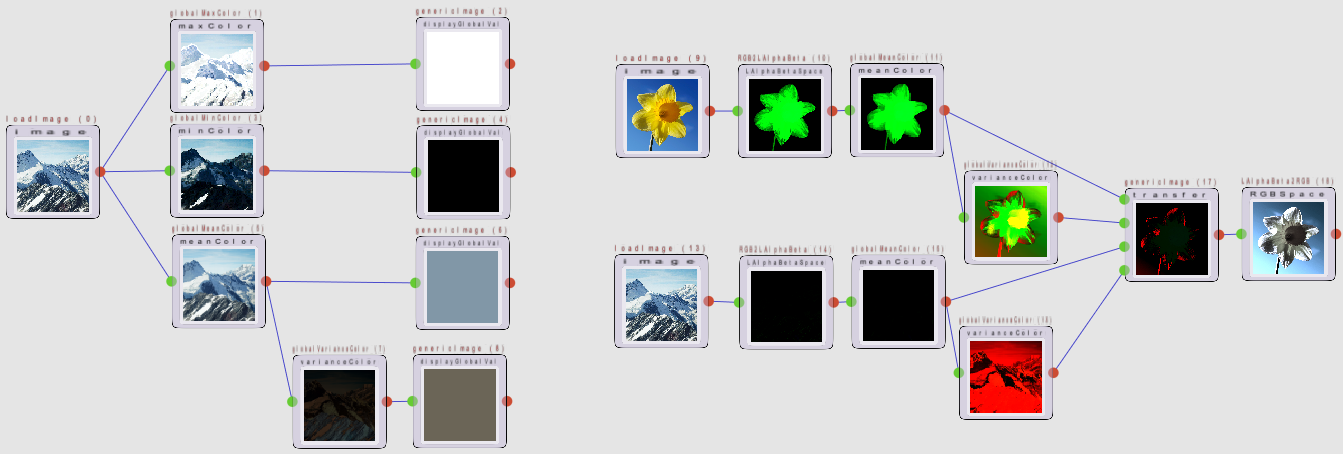
\includegraphics[width=\linewidth]{imgs/pipe-global.png} 
  \caption{\label{fig:pipe-global}Global values pipeline example.}
\end{figure}
%
\noindent The pipeline shown in Fig.~\ref{fig:pipe-global} also makes use of
pyramid nodes to compute global values on images such as the
minimum/maximum/mean/variance colors. This is shown on the left, where
generic images nodes are used to access the last levels of the
pyramids and visualize the corresponding colors. On the right side,
the mean and standard deviations are used to reshape the histogram of
a source image based on a target one (a simple example-based color
transfer function).

\addsubsection{histograms.gra}
%
\begin{figure}[htb]
  \centering 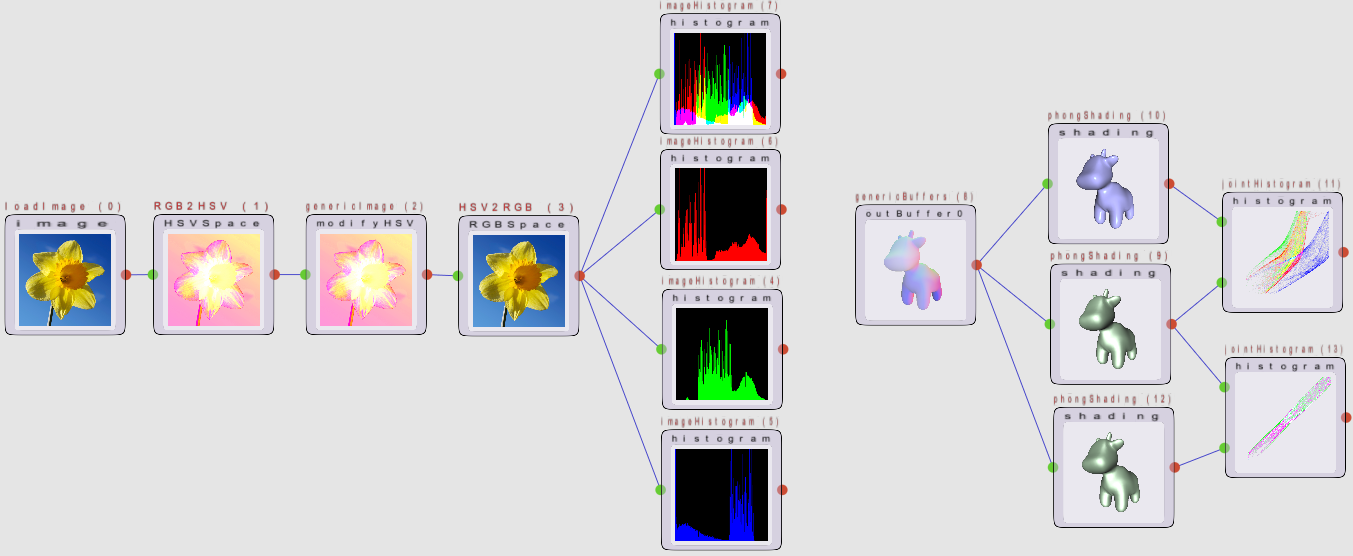
\includegraphics[width=\linewidth]{imgs/pipe-hist.png} 
  \caption{\label{fig:pipe-hist}Histograms pipeline example.}
\end{figure}
%
\noindent Histograms (Fig.~\ref{fig:pipe-hist}) are based on generic splat
nodes. The left side of the figure shows the original node as well as
some variations that select only one particular channel to
display. The geometry shader was slightly modified for this
purpose. Histograms are obtained in real-time. Try to play with the
parameters of the ``modifyHSV'' node to visualize their effects. On
the right side, a joint histogram is used to visualize the
correlations between 2 rendered images.


\addsubsection{poisson-diffusion.gra}
%
\begin{figure}[htb]
  \centering 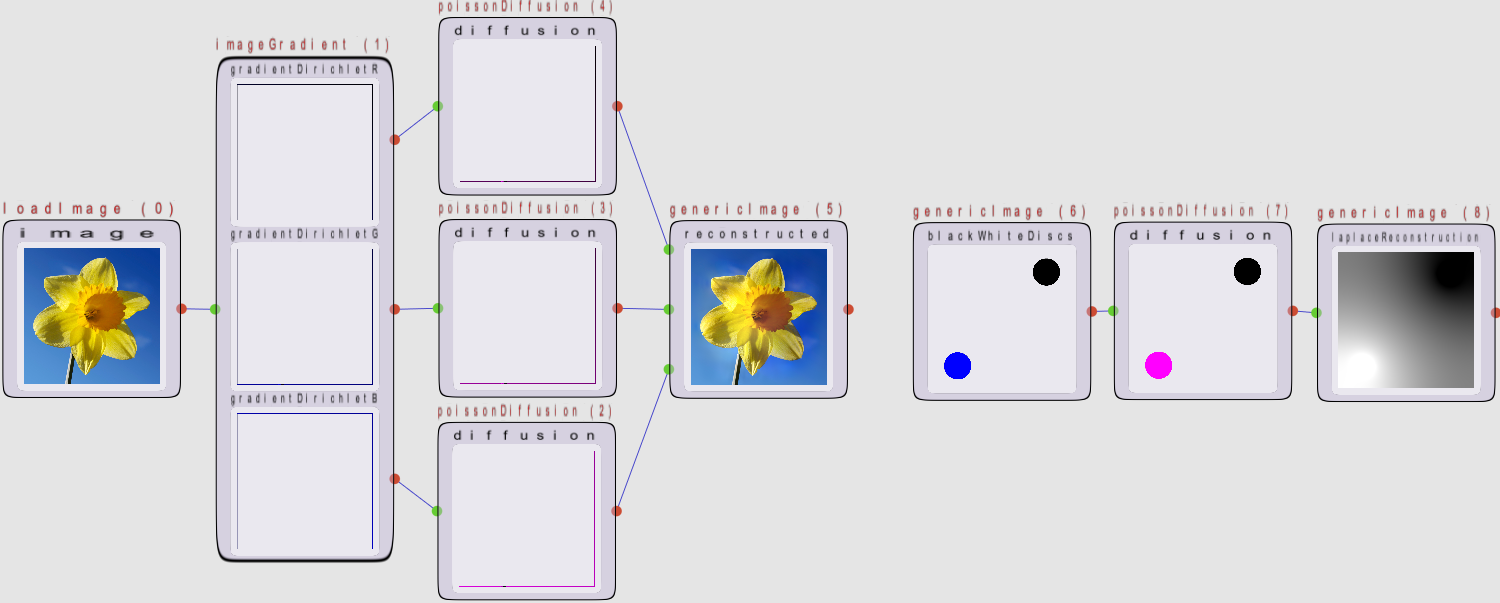
\includegraphics[width=\linewidth]{imgs/pipe-poisson.png} 
  \caption{\label{fig:pipe-poisson}Diffusion pipeline example.}
\end{figure}
%
\noindent The pipeline shown in Fig.~\ref{fig:pipe-poisson} illustrates the use
of the poisson diffusion node to reconstruct an image from its
gradients. On the left, 3 diffusions are computed (one for each
channel) to compute the image. The ``gradientDirichlet node'' is based
on a generic image node and computes the image gradient for each
channel, as well as some Dirichlet constraints on the borders (to
avoid offset differences in the result). The second example on the
right shows how to use the poisson node to compute a laplacian
diffusion. In that case, the gradient is set to 0 everywhere. Only
Dirichlet constraints are placed inside the 2 black/white discs. The
node then diffuses the data by minimizing the gradient. The positions
of the discs can be controlled in real-time in the viewer: click on the
blackWhiteDiscs image, press ``space'' and modify the position of the discs
with the mouse.

\addsubsection{renderings.gra}
%
\begin{figure}[htb]
  \centering 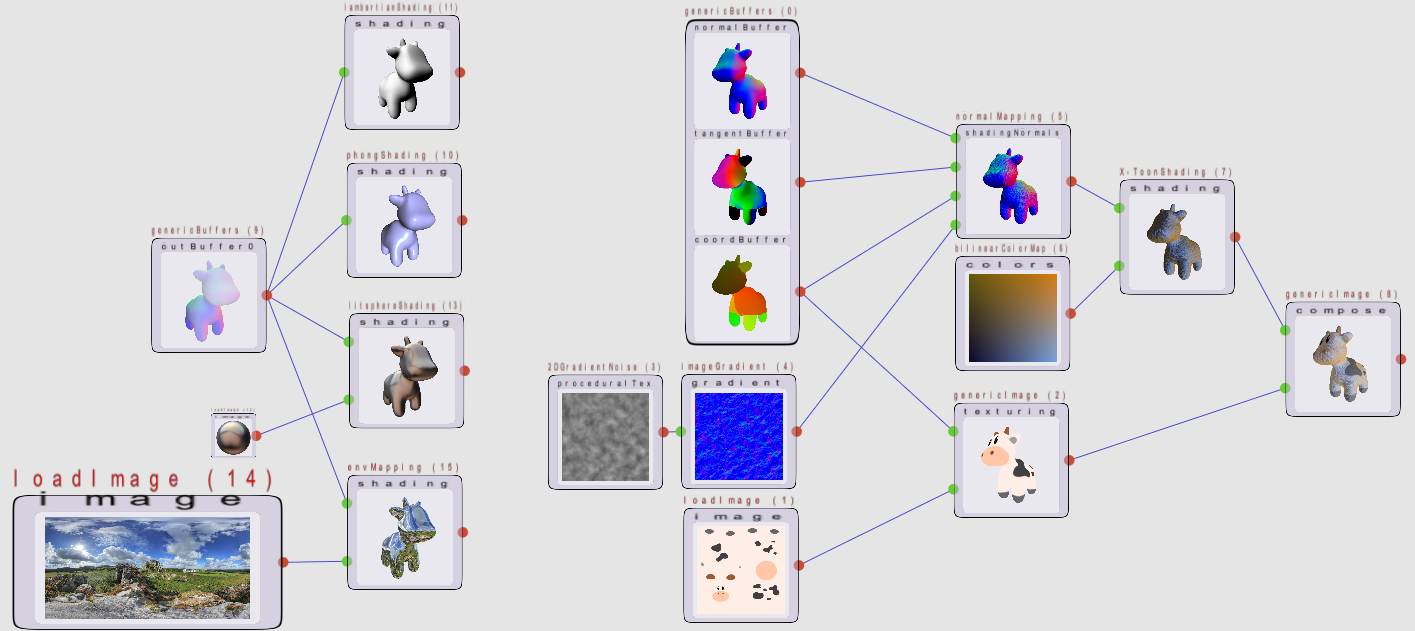
\includegraphics[width=\linewidth]{imgs/pipe-rend.png} 
  \caption{\label{fig:pipe-rend}Renderings pipeline example.}
\end{figure}
%
The rendering pipeline (Fig.~\ref{fig:pipe-rend}) shows the available
shading nodes on the left. They can all be controlled via the mouse
(for moving the light direction) or via some parameters inside the
interface. The right example starts from a generic buffer node for
loading the cow model, and uses the texture coordinates as well as the
tangents in order to perturb normal at the surface (normal-mapping
technique). The model texture is also loaded and combined with a
simple shading to obtain the final result on the right. Parameters for
the normal perturbation, shading colors and textures might be modified
inside the corresponding node interfaces.

\newpage
\addsubsection{displacement-mapping.gra}
%
\begin{figure}[htb]
  \centering 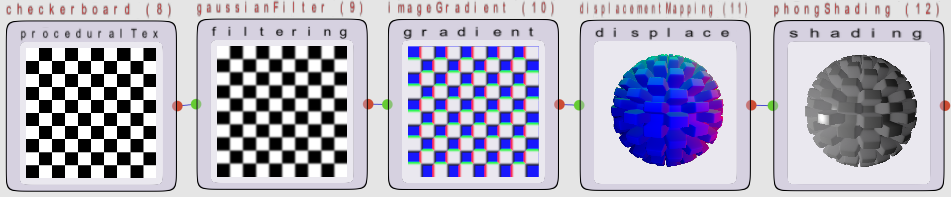
\includegraphics[width=\linewidth]{imgs/pipe-displace.png} 
  \caption{\label{fig:pipe-displace}Displacement mapping pipeline example.}
\end{figure}
%
The displacement mapping technique (Fig.~\ref{fig:pipe-displace})
displaces mesh vertices based on an input height map. Here,
the input texture also contains the associated normals, based on
the gradient of a blurred checkerboard texture. The displacement is
applied on a sphere. The ``disp'' parameter inside the interface of
the displacement node controls how the sphere is deformed. ``T''
controls how the sphere should be tesselated (how many triangles
needed) via the tesselation shader to displace all the details.


\addsubsection{animate.gra}
%%
%\begin{figure}[tbh]
%  \centering 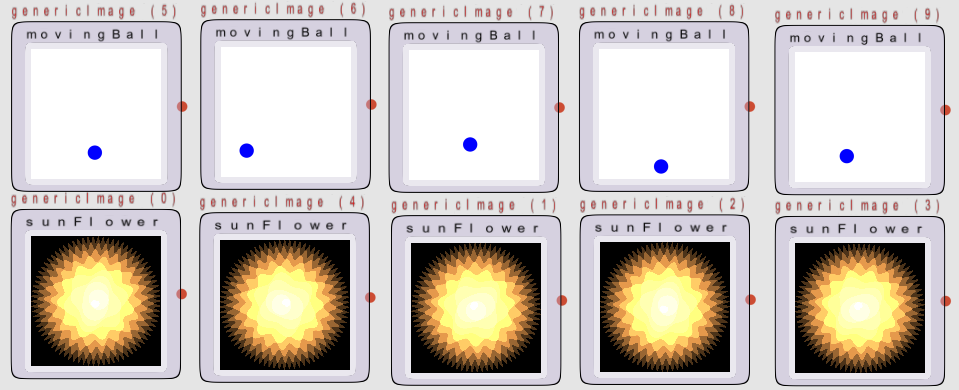
\includegraphics[width=\linewidth]{imgs/pipe-anim.png} 
%  \caption{\label{fig:pipe-anim}The animation pipeline example.}
%\end{figure}
%%
The animation example illustrates basic animation behaviors. 
You will have to open the pipeline to follow the remainder of this section. 
The five nodes on the top row show a disc passing through 4 control points, using five different interpolation types: linear, step, shepard, spline and hermite. 
The second row of nodes shows a rotated sunFlower illustrating the effect of the curve behavior on a small
number of control points: no behavior (all linear), constant, repeat, mirrored repeat and offseted repeat. 
Press the ``p'' key to start the animation and see the effects (press
``shift+p'' to stop it). To check and modify the curves, click on the
editing button of the parameter inside the interface of the node.


\addsubsection{fourier-transform.gra}

\begin{figure}[tbh]
 \centering 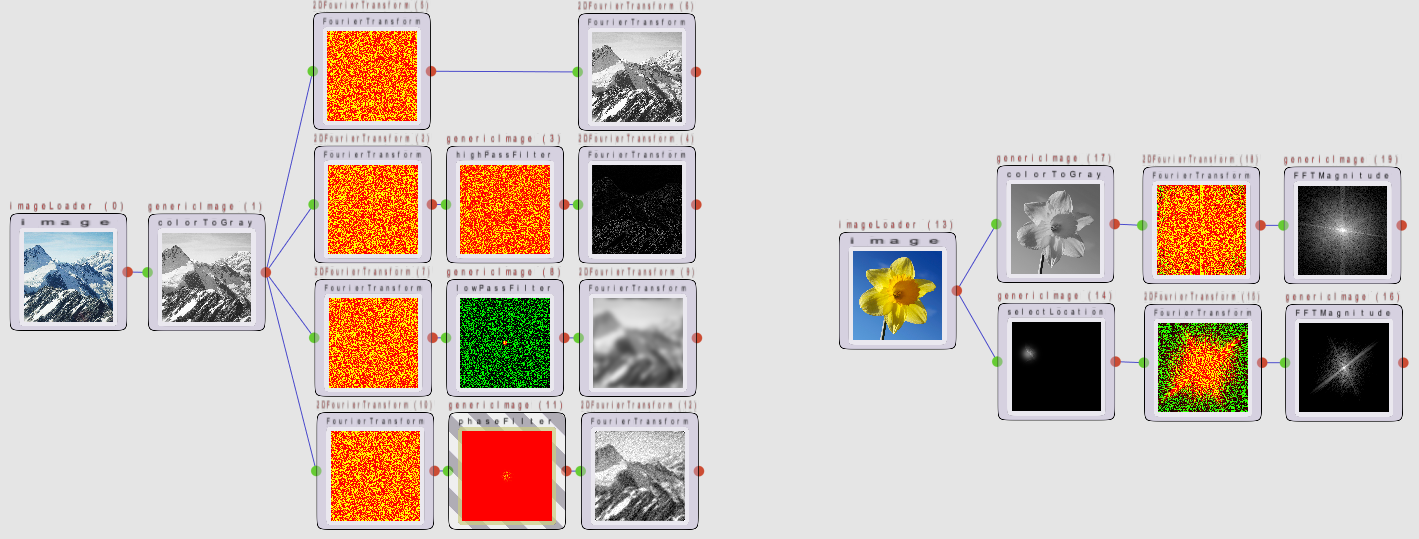
\includegraphics[width=\linewidth]{imgs/pipe-fourier.png} 
 \caption{\label{fig:pipe-fourier}The Fourier pipeline example.}
\end{figure}

The Fourier transform example (Fig.~\ref{fig:pipe-fourier}) shows how
to use the node to manipulate the frequency content in images. On the
left, forward and backward Fourier transforms are successively
applied. From top to bottom: the original image is reconstructed; a
highpass filter is applied (using a genericImage node that multiplies
the frequency magnitude with a user-defined gaussian function); a
low-pass filter is applied (on the magnitude - same approach); a
low-pass filter is applied (on the phase - same approach). On the
right, the magnitude is rescaled using a generic node to visualize the
spectrum. (top) the full spectrum is visualized; (bottom) the user can
interact with the select node (click + space on the node and interact
in the viewer) to visualize the spectrum of a part of the image only.

